%
% beugung-herleitung.tex -- Herleitung aus WsComm2-Vorlesung
%
%
% !TEX root = ../../buch.tex
% !TEX encoding = UTF-8
%

\section{Anwendungsbeispiel}
\kopfrechts{Anwendungsbeispiel}

In der Drahtloskommunikation werden die Fresnel-Integrale für 
die Beugung von Signalen an einer Knife-Edge gebraucht. %TODO: Bild Knife-Edge
Zwischen zwei Antennen ragt ein Hindernis in die direkte 
Linie von Sender und Empfänger. 
Nun wird jede ausgesendete Welle als Wavelet angesehen,
welche sich nach Huygens kreisförmig ausbreitet. 
Um die Beugung zu berechnen, 
bedarf es einiger Definitionen, 
welche im weiteren Verlauf verwendet werden und in 
Abbildung~\ref{fresnel:Pythagoras-Bild} ersichtlich sind:
\begin{itemize}
    \item 
    $d$ sei der Abstand vom Empfänger zur Knife-Edge
    \item 
    $h$ sei die Höhe eines Wavelets direkt über der Knife-Edge
    \item
    $h_{edge}$ sei die Höhe, welche die Knife-Edge in die direkte Linie zwischen Sender und Empfänger hineinragt
    \item 
    $r$ sei die Distanz eines Wavelets zum Empfänger
\end{itemize}

\begin{figure} % TODO: evtl. durch tikz ersetzen
    \centering
    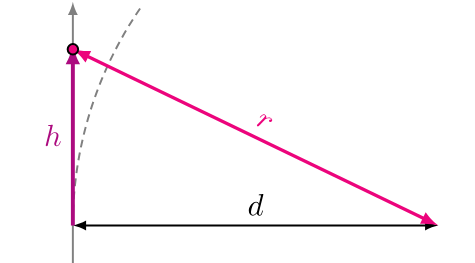
\includegraphics[width=0.8\linewidth]{papers/fresnel/images/Pythagoras-Dreieck.png}
    \caption{
        Definitionen für die Berechnung
        \label{fresnel:Pythagoras-Bild}
    }
\end{figure}

\subsection{Fresnel-Integrale}
Die Fresnel-Integrale werden hier in der Form
\begin{equation}
    C(v) 
    = 
    \int_{0}^{x} \cos \left(\frac{\pi}{2}t^2\right)
    \quad \text{und} \quad
    S(v) 
    = 
    \int_{0}^{x} \sin \left(\frac{\pi}{2}t^2\right)
    \label{fresnel:integral-C-S}
\end{equation}
definiert, wobei
\[
C(\infty)
=
S(\infty)
=
\frac{1}{2}
\quad
\text{und}
\quad
C(-a)
=
-C(a)
\]
sei.

\subsection{Fresnel Approximation}
Mittels Pythagoras geht hervor, dass 
\[
r 
= 
\sqrt{d^2 + h^2}
=
d \sqrt{1 + \frac{h^2}{d^2}}
\]
und mittels Taylor-Approximation für $d \gg h$
\[
r 
=
d \sqrt{1 + \frac{h^2}{d^2}}
\sim
d \left( 1 + \frac{h^2}{2d^2} \right)
=
d + \frac{h^2}{2d},
\]
unter der Annahme, dass in den meisten Fällen die Distanz zur Knife-Edge um einige Magnituden grösser ist,
als die Höhe der Wavelets.
Will man nun das Signal zweier ankommender Wavelets am Empfänger berechnen, geht dies durch Einsetzen
\begin{align*}
    \text{für } h = 0: \quad \psi_0
    &=
    \psi \cdot \frac{\mathrm{e}^{-jkr_0}}{r_0}
    =
    \psi \cdot \frac{\mathrm{e}^{-jkd}}{d},
    \\
    \text{für } h = h: \quad \psi_1
    &=
    \psi \cdot \frac{\mathrm{e}^{-jkr_1}}{r_1}
    \approx
    \psi \cdot \frac{\mathrm{e}^{-jk\left(d+\frac{h^2}{2d}\right)}}{d}.
\end{align*}
Da dieses Vorgehen eine Approximation ist, 
werden Abschwächungen und Verzögerungen der Signale vernächlässigt
$\to$ keine Faktoren wie $1/r, 1/d$ und $\omega t$. Daraus ergibt sich
\[
\psi (r,t)
=
\psi_0 \cdot \frac{\mathrm{e}^{j(\omega t - kr)}}{r}
\quad \to \quad
\psi_0 \cdot \mathrm{e}^{-jkr}
=
\psi (r)
\]
und kann für Wavelets in verschiedenen Höhen mit $h = h_i$ als
\[
\psi_i
=
\psi \cdot \mathrm{e}^{-jkr}
\approx
\psi \cdot \mathrm{e}^{-jk\left(d+\frac{h^2_i}{2d}\right)}
\]
dargestellt werden. Mittels Superposition folgt
\[
\psi_{rx}
=
\sum_i \psi_i
=
\sum_i \psi \cdot \mathrm{e}^{-jkr}
=
\psi \cdot \sum_i \mathrm{e}^{-jk\left(d+\frac{h^2_i}{2d}\right)}
=
\underbrace{\psi \cdot \mathrm{e}^{-jkd}}_{=\psi_0} \sum_i \mathrm{e}^{-jk\left(\frac{h^2_i}{2d}\right)}
\]
und mittels Wellendichte $\rho_{\psi} = \frac{d\psi}{dh} \Rightarrow \psi = \rho_{\psi} \Delta h $
\[
\psi_{rx}
=
\psi_0 \cdot \sum_i \mathrm{e}^{-jk\left(\frac{h^2_i}{2d}\right)}
=
\rho_{\psi_0} \cdot \sum_i \mathrm{e}^{-jk\left(\frac{h^2_i}{2d}\right)} \Delta h,
\]
welches anschliessend mittels $\Delta h \to dh$ zum Integral
\[
\psi_{rx}
=
\rho_{\psi_0} \int_{h_{edge}}^{\infty} \mathrm{e}^{-jk\left(\frac{h^2}{2d}\right)} dh
=
\rho_{\psi_0} \int_{h_{edge}}^{\infty} \left(\cos \frac{kh^2}{2d} - j \sin \frac{kh^2}{2d}\right) dh
\]
wird.
Dies kann mit den gängigen Regeln in zwei Integrale mit Beginn bei 0 umgestellt werden, was zu
\begin{align*}
    \psi_{rx}
    &=
    \rho_{\psi_0} \int_{h_{edge}}^{\infty} \left(\cos \frac{kh^2}{2d} - j \sin \frac{kh^2}{2d}\right) dh
    \\
    &=
    \underbrace{\rho_{\psi_0} \int_{0}^{\infty} \left(\cos \frac{kh^2}{2d} - j \sin \frac{kh^2}{2d}\right) dh}_{\text{Gesamte Wellendichte}}
    -
    \underbrace{\rho_{\psi_0} \int_{0}^{h_{edge}} \left(\cos \frac{kh^2}{2d} - j \sin \frac{kh^2}{2d}\right) dh}_{\text{Verlorene Wellendichte durch Knife-Edge}}  
\end{align*}
führt.
Das Integral ähnelt C aus der Formel~\eqref{fresnel:integral-C-S} und kann mittels der Substitution
\[
h
\to
t(h)
=
h\sqrt{\frac{h}{\pi d}}
\Rightarrow
\frac{dh}{dt}
=
\sqrt{\frac{\pi d}{k}}
\Rightarrow
dh
=
\sqrt{\frac{\pi d}{k}} dt
\]
aufgelöst werden zu
\begin{equation*}
    \int_{0}^{h_{edge}} \cos \left(\frac{k}{2d}h^2\right) dh
    =
    \sqrt{\frac{\pi d}{k}} \int_{0}^{h_{edge}\sqrt{\frac{k}{\pi d}}} \cos \left(\frac{\pi}{2}t^2\right) dt
    =
    \sqrt{\frac{\pi d}{k}} C(v).
\end{equation*}
Über das ganze Integral ergibt sich
\begin{equation}
    \psi_{rx} (v)
    =
    \rho_{\psi_0} \sqrt{\frac{\pi d}{k}} \cdot \left[\frac{1}{2} - C(v) -j\left(\frac{1}{2}-S(v)\right)\right]
\end{equation}
mit dem daraus entstehenden Fresnel-Parameter
\begin{equation}
    v
    =
    h_{edge} \sqrt{\frac{k}{\pi d}}
    \quad
    \overset{k = \frac{2 \pi}{\lambda}}{=}
    \quad
    h_{edge} \sqrt{\frac{2}{\lambda d}}.
\end{equation}

\subsection{Beugungsverlust}
Aus den hervorgehenden Gleichungen kann der Beugungsverlust $L(v)$ berechnet werden, indem
\begin{equation}
    L(v)
    =
    \frac{|\psi_{rx} (-\infty)|^2}{|\psi_{rx} (v)|^2}
    =
    \dots
    =
    \frac{2}{\left|\frac{1}{2}-C(v)\right|^2 + \left|\frac{1}{2}-S(v)\right|^2}
    \label{fresnel:diff-loss-einseitig}
\end{equation}
und für $L_{dB}$ die Umrechnung
\[
L_{dB} (v)
=
10 \cdot \log_{10}L(v)
\]
anwendet.

%TODO: Bild für beidseitige Diff-Loss
Die Gleichung \eqref{fresnel:diff-loss-einseitig} gilt für Verluste zwischen Knife-Edge und Empfänger. 
Soll nun der Beugungsverlust zwischen Sender und Empfänger mit dazwischenliegender Knife-Edge wie in Abbildung~\ref{fresnel:diff-loss-beidseitig} berechnet
werden, kann der Fresnel-Parameter so erweitert % Parameter bleibt, wenn einer der Stationen viel weiter vom Knife-Edge weg ist, als der andere
\footnote{Die Substitution lautet $\frac{1}{d} \to \frac{d_1 + d_2}{d_1d_2}$, die Herleitung ist dem Leser überlassen} 
werden, dass
\begin{equation}
    v
    =
    h_{edge} \sqrt{2\frac{d_1 + d_2}{\lambda d_1 d_2}}.
\end{equation}

\begin{figure}
    \centering
    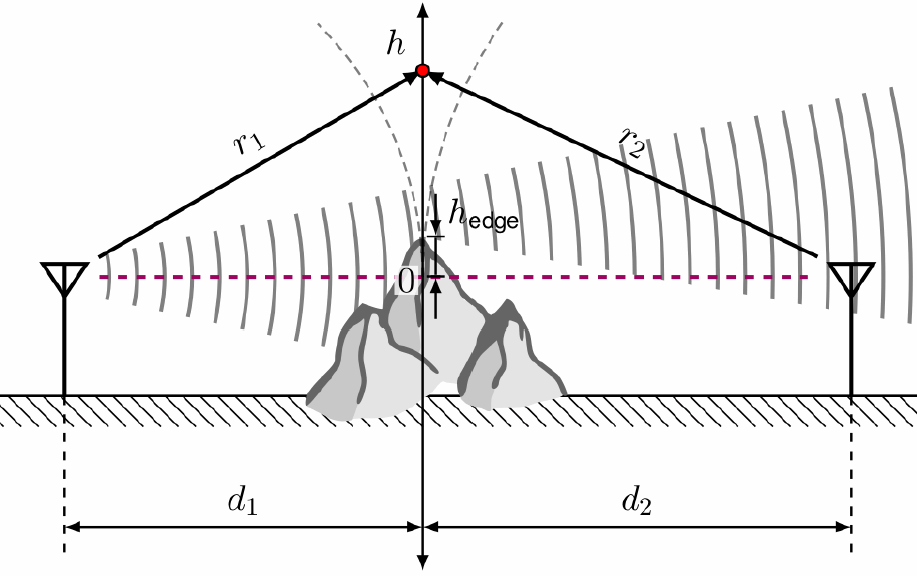
\includegraphics[width=0.8\linewidth]{papers/fresnel/images/Diff-Loss_beidseitig.png}
    \caption{
        Dartsellung der Verluste zwischen Sender und Empfänger
        \label{fresnel:diff-loss-beidseitig}
    }
\end{figure}

Die daraus resultierenden Verluste $L_{dB}$ können aus Abbildung~\ref{fresnel:Fresnel-Diagram}
ausgelesen oder mit folgenden Formeln
\begin{subequations}
    \begin{align}
        v > 1: \quad
        -L_{dB}
        &=
        20 \log_{10}v + 13 dB
        \\
        v > -0.7: \quad
        -L_{dB}
        &=
        20 \log_{10}\left(\sqrt{(v-0.1)^2 + 1} + v -0.1\right) + 6.9 dB
        \\
        \text{sonst:} \quad
        -L_{dB}
        &=
        10 \log_{10} L(v)
    \end{align}
\end{subequations}
angenähert werden.

\begin{figure}
    \centering
    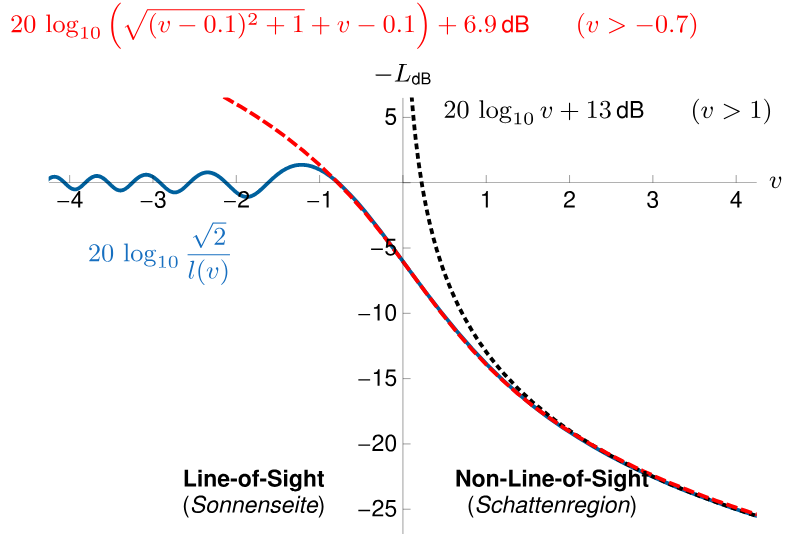
\includegraphics[width=0.8\linewidth]{papers/fresnel/images/Fresnel-Diagram.png}
    \caption{
        Diagramm Fresnel-Parameter und Verluste
        \label{fresnel:Fresnel-Diagram}
    }
\end{figure}